\documentclass{ximera}
\author{Jont Allen}
\begin{document}
\begin{problem}
    Consider the functions \(f(s) = s^2 + 6s + 25\) and \(g(s) = s^2 + 6s + 5\).
    
    Find the zeros of \(f(s)\) and \(g(s)\) using the command \texttt{roots()}.
    \[
    \text{Zeros of } f(s): \answer{-3} \pm \left(\answer{4}\right)i
    \]
    and give the answers in order from least to greatest below:
    \[
    \text{Zeros of } g(s): \answer{-5}, \answer{-1}
    \]
    \begin{feedback}[correct]
    The roots of \(f(s)\) are \(-3 \pm 4i\) (in MATLAB: \texttt{roots([1 6 25])}). The roots of \(g(s)\) are \(-1\) and \(-5\) (in MATLAB: \texttt{roots([1 6 5])}).
    \end{feedback}
\end{problem}

\begin{problem}
    Show the roots of \(f(s)\) as red circles and of \(g(s)\) as blue plus signs.
    Label the x-axis as ``Real Part'' and the y-axis as ``Imaginary Part.'' Use \texttt{hold on} and \texttt{grid on} when plotting.
\begin{center}
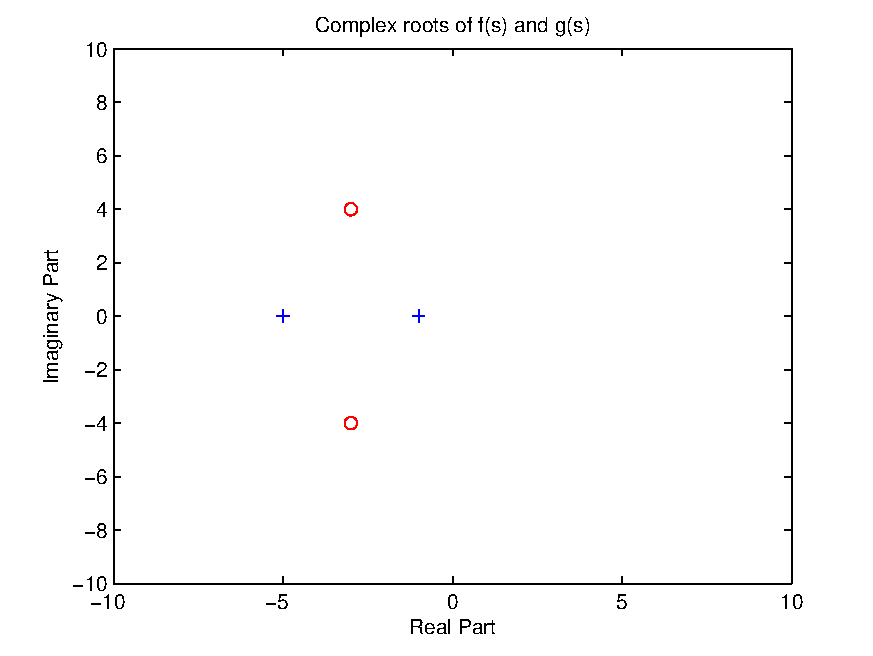
\includegraphics{hw1_1_1bc-eps-converted-to.pdf}
\end{center}
\end{center}
    \begin{feedback}[correct]
    Use MATLAB/Octave commands to plot the roots of \(f(s)\) and \(g(s)\) on a complex plane, with appropriate labels and a grid.
    \end{feedback}
\end{problem}

\begin{problem}
    Give the plot the title ``Complex Roots of \(f(s)\) and \(g(s)\).'' Use \texttt{xlabel}, \texttt{ylabel}, \texttt{xlim([-10 10])}, and \texttt{ylim([-10 10])}.
    \begin{multipleChoice}
        \choice[correct]{I've done this.}
        \choice{I have not done this.}
    \end{multipleChoice}
    \end{multipleChoice}
    \begin{feedback}[correct]
    Ensure the plot includes proper limits and titles for a complete visualization.
    \end{feedback}
\end{problem}
\end{document}
